\documentclass[a4paper,11pt]{article}

\usepackage[utf8]{inputenc}
\usepackage[swedish]{babel}

\usepackage{graphicx}
\usepackage{semantic}
\usepackage{minted}
\usepackage{fancyvrb}

\begin{document}

\title{
  \textbf{Huffman\\
  \small Programmering II}
}
\author{Axel Karlsson}
\date{VT22 \today}

\maketitle

\section*{Inledning}
I denna rapport ska jag redovisa min lösning för uppgift 12, Huffman. Jag har skapat ett program som kan komprimera text med huffmankodning och sedan testat programmets prestanda med olika typer av texter. 


\section*{Frekvens av chars}
Denna funktion skulle hitta hur många gånger varje unik {\tt char} förekom i en textsträng. Jag implementerade detta genom funktionen {\tt freq/1}. Funktionen går igenom varje index i en sträng (alltså en lista av {\tt chars}) och sparar antalet gånger ett tecken förekommer som en tuppel i en ackumulatorlista. Jag har använt funktioner från {\tt List} modulen (även i den utelämnade koden), så det är inte självklart vilken komplexitet funktionen har.

\begin{minted}{elixir}
  def freq(sample) do freq(sample, []) end # Anropa med ackumulator
  def freq([], freq) do freq end # Alla chars är kollade
  def freq([char | rest], freq) do
    case List.keymember?(freq, char, 0) do
      true ->
        # <Inkrementera indexet i freq>
      false ->
        # <Lägg till {char, 1} i freq>
    end
  end
\end{minted}
Funktionen returnerar en lista av tupplar, se nedan.
\begin{minted}{elixir}
  [
    {100, 1}, # {<asciivärde>, <antal förekomster>}
    ...
    {115, 1}
  ]
\end{minted}

\section*{Huffmanträd}
Nästa del av uppgiften var att skapa ett huffmanträd utifrån resultatet av {\tt freq/1}. Den givna algoritmen för att göra detta var att ta de två lägsta värdena i frekvenslistan, kombinera dem till ett och sedan stoppa in dem igen. Detta upprepas tills det endast finns ett element i listan, som då kommer vara roten till ett träd.\\
Jag implementerade detta i funktionen {\tt huffman/1}. Funktionen tar en lista av tupplar, som den från {\tt freq/1}, och sorterar den med minsta elementet först.

\begin{minted}{elixir}
  def huffman(freq) do
    freq = List.keysort(freq, 1) # Sortera listan av chars efter frekvens
    hufftree(freq)
  end
\end{minted}

Denna lista bearbetas sedan i funktionen {\tt hufftree/1}, som bygger trädet med den tidigare nämnda algoritmen. Återigen använde jag {\tt List} modulen.

\begin{minted}{elixir}
  def hufftree([root]) do root end # När det endast finns ett element
  def hufftree(tree) do
    {el1 = {_, n1}, tree} = List.pop_at(tree, 0) # Första elementet
    {el2 = {_, n2}, tree} = List.pop_at(tree, 0) # Andra elementet
    comb = {{el1, el2}, n1+n2} # Kombinera dem
    tree = insert_sorted(comb, tree) # Stoppa in på rätt plats
    hufftree(tree)
  end
\end{minted}

\section*{Kodningstabeller}
Det sista steget som krävdes för att koda text var en funktion som skapar en kodningstabell utifrån ett huffmanträd. Denna tabell innehåller information om hur man ska navigera trädet för att nå en viss {\tt char}.\\
Funktionen implementerades i {\tt encode\_table/1}. Den använder två ackumulatorlistor, en för tabellen och en för vägen. Funktionen går rekursivt igenom hela trädet och varje gång ett löv, alltså en {\tt char}, nås sparas vägen till det i tabellen.

\begin{minted}{elixir}
  def encode_table(tree) do encode_table(tree, [], []) end
  # Matchar mot en gren
  def encode_table({{el1, el2}, _n}, table, path) do
    table = encode_table(el1, table, path ++ [1])
    table = encode_table(el2, table, path ++ [0])
    table
  end
  # Matchar mot ett löv
  def encode_table({el, _n}, table, path) do table ++ [{el, path}] end
\end{minted}
Detta resulterar i en datastruktur som den nedan.
\begin{minted}{elixir}
[
  {122, [1, 1, 1]},
  ...
  {101, [0, 0, 0]}
]  
\end{minted}

\section*{Kodning och avkodning}
De tidigare nämnda funktionerna kombinerades i funktionerna {\tt encode/2} och {\tt decode/2}. Den första funktionen går igenom varje {\tt char} i den givna texten, kollar upp det motsvarande värdet i kodningstabellen och sparar det i en ackumulatorlista som sedan returneras.

\begin{minted}{elixir}
  def encode([], _table) do [] end
  def encode([char | rest], table) do
    {_, path}  = List.keyfind!(table, char, 0)
    path ++ encode(rest, table)
  end
\end{minted}

Funktionen för avkodning var i princip given i uppgiften så jag har valt att inte inkludera koden.

\section*{Benchmarks}
Jag testade funktionerna {\tt freq/1}, {\tt huffman/1}, {\tt encode/2} och {\tt decode/2} för olika textlängder och med vissa tecken filtrerade. Funktionen {\tt bench/1} väljer {\tt i * size} tecken ur en given text. Denna text skickas sedan till {\tt bench\_huff/1} som mäter exekveringstiden på de fyra tidigare nämnda funktionerna med texten. Denna mätning görs 100 gånger för varje {\tt i}, och genomsnittet av resultaten returneras.\\
Texten jag använde var en engelsk version av Mary Shelleys Frankenstein på cirka fyrahundratusen tecken. Jag gjorde även mätningar där jag filtrerade ut alla tecken utom de 10, 8, 5 och 3 vanligaste tecknen.

\begin{minted}{elixir}
  def bench(file) do
  text = read(file, :all)
  ... # Här filtreras texten
    for i <- 1..200 do
      # <Välj i*100 tecken på en slumpmässig plats i texten>
      {t_fr, t_tr, t_en, t_de} = loop(fn() -> bench_huff(text) end)
      ...
    end
    :ok  
  end    
\end{minted}

\section*{Resultat}
\begin{figure}[H]
  \begin{centering}
    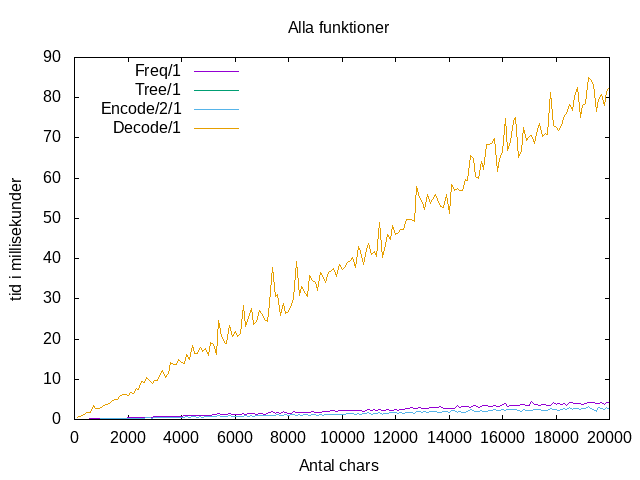
\includegraphics[scale=0.6]{images/20_000_regular.png}
    \caption{Benchmark av alla funktioner}
    \label{fig:bench_all}
  \end{centering}
\end{figure}

\begin{figure}[H]
  \begin{centering}
    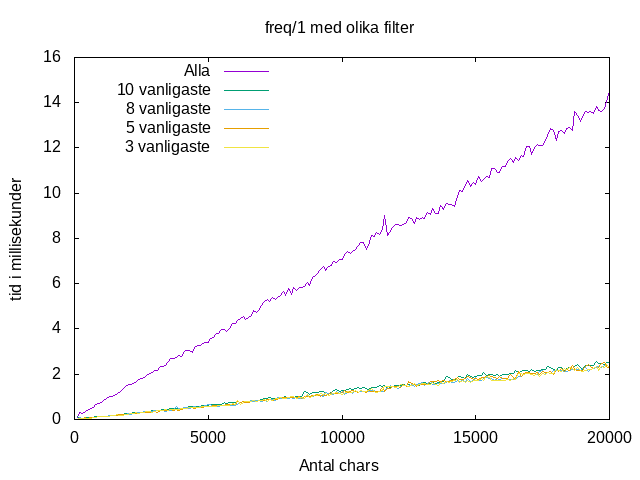
\includegraphics[scale=0.6]{images/20_000_freq.png}
    \caption{Benchmark av freq/1. De olika graferna är olika filtreringar av texten.}
    \label{fig:bench_freq}
  \end{centering}
\end{figure}

\begin{figure}[H]
  \begin{centering}
    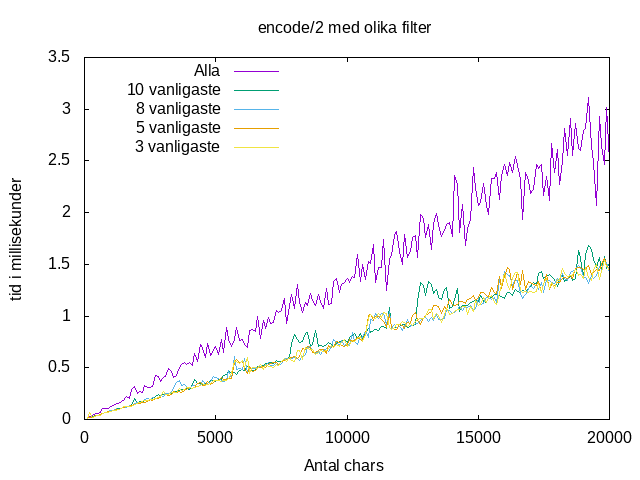
\includegraphics[scale=0.6]{images/20_000_encode.png}
    \caption{Benchmark av encode/2. De olika graferna är olika filtreringar av texten.}
    \label{fig:bench_encode}
  \end{centering}
\end{figure}

\begin{figure}[H]
  \begin{centering}
    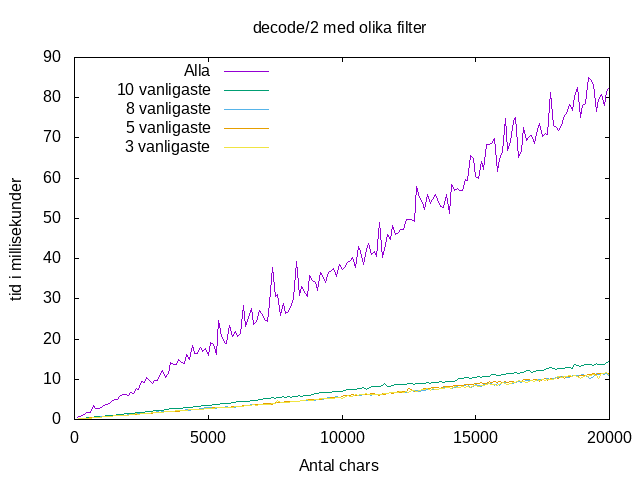
\includegraphics[scale=0.6]{images/20_000_decode.png}
    \caption{Benchmark av decode/2. De olika graferna är olika filtreringar av texten.}
    \label{fig:bench_decode}
  \end{centering}
\end{figure}

\section*{Analys}
I figurer \ref{fig:bench_freq}, \ref{fig:bench_decode} och \ref{fig:bench_encode} syns ett starkt samband mellan antal unika element i texten och exekveringstid. Alla tre funktioner som mäts i graferna innehåller ett anrop till {\tt List.keyfind/3} i en lista vars längd beror på antal unika element, vilket jag skulle gissa är anledningen till dessa tre liknande resultat.\\
I figur \ref{fig:bench_all} ser vi att {\tt decode/2} är den långsammaste funktionen med stor marginal. Jag tror att det beror på det tidigare nämnda anropet till {\tt List.keyfind/3}. I {\tt decode/2} sker ett sådant anrop för varje bit i den huffmankodade texten, medan det i {\tt freq/1} och {\tt encode/2} sker ett anrop för varje {\tt char} i texten. Då varje {\tt char} kodas till åtminstonne en bit blir det totalt många fler anrop.
\end{document}
